\documentclass[aspectratio=43]{beamer}
\usetheme{Berlin}

\usepackage[czech]{babel}
\usecolortheme{dolphin}
\definecolor{accent}{HTML}{559915}
\setbeamercolor{structure}{fg=accent}
\usepackage{graphicx}
\usepackage{dirtree}
\usepackage{listings}
\usepackage[T1]{fontenc}
\usepackage{lmodern}
\usepackage[utf8]{inputenc}
\usepackage{caption}
\usepackage{bbding}
\usepackage{xurl}
\usepackage{scrextend}
\usepackage{minted}
\usepackage{appendixnumberbeamer}

\captionsetup{labelformat=empty}

\beamertemplatenavigationsymbolsempty
\defbeamertemplate*{title page}{customized}[1][]
{
	\begin{center}
	\usebeamerfont{title}\inserttitle\par
	\usebeamerfont{subtitle}\insertsubtitle\par
	\vspace{1cm}
	\def\svgwidth{\columnwidth}\scalebox{0.25}{\input{../img/BElogo.pdf_tex}}
	\end{center}
	\vfill
	\usebeamercolor[fg]{subtitle}
	\usebeamerfont{author}\insertauthor\par
	\usebeamerfont{institute}\insertinstitute\par
	\usebeamerfont{date}\insertdate\par
	\usebeamercolor[fg]{titlegraphic}\inserttitlegraphic
}

\hypersetup{unicode}
\hypersetup{breaklinks=true}


\title{BookExchange}
\subtitle{Bazar Učebnic Arabská}
\author{Josef Litoš 4.E}
\date{}
\institute{Gymnázium, Praha 6, Arabská 14}
\setbeamertemplate{sidebar right}{}
\setbeamertemplate{footline}{%
\hfill\textbf{\insertframenumber{} / \inserttotalframenumber} \hspace{0.01cm} \vspace{0.1cm}}
\setbeamerfont{footnote}{size=\tiny}

\begin{document}

\begin{frame}[plain]
	\maketitle
\end{frame}

\clearpage
\setcounter{framenumber}{0}

\frame{
	\frametitle{Vznik}
	\section{Vznik}
	\begin{itemize}
		\item Období karantény
		\item zrušení burzy
		\item učebnice se hromadí
	\end{itemize}
}

\section{Rozvržení}
\frame{
	\frametitle{Prostředky}
	\begin{itemize}
		\item MariaDB
		\item ExpressJS, nodemailer, handlebars
		\item passport, mariadb, multer
		\item ReactJS, axios, MaterialUI, client-compress
	\end{itemize}
}

\frame{
	\frametitle{Propojení}
	\centering
	\vspace{1cm}
	\scalebox{1.5}{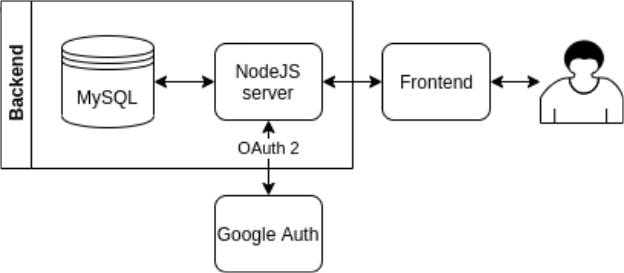
\includegraphics{../img/propojeni.png}}
}

\frame{
	\frametitle{Databáze}
	\section{Databáze}
	\centering
	\def\svgwidth{\columnwidth}\scalebox{0.7}{\input{../img/ER_Diagram.pdf_tex}}
}

\section{Server}
\frame{
	\frametitle{Struktura}
	\begin{itemize}
		\item routes
		\item services
		\item mails
		\item app.js
	\end{itemize}
}
\frame{
	\frametitle{RestAPI}
	\begin{columns}
		\begin{column}{.45\textwidth}
			\scalebox{0.5}{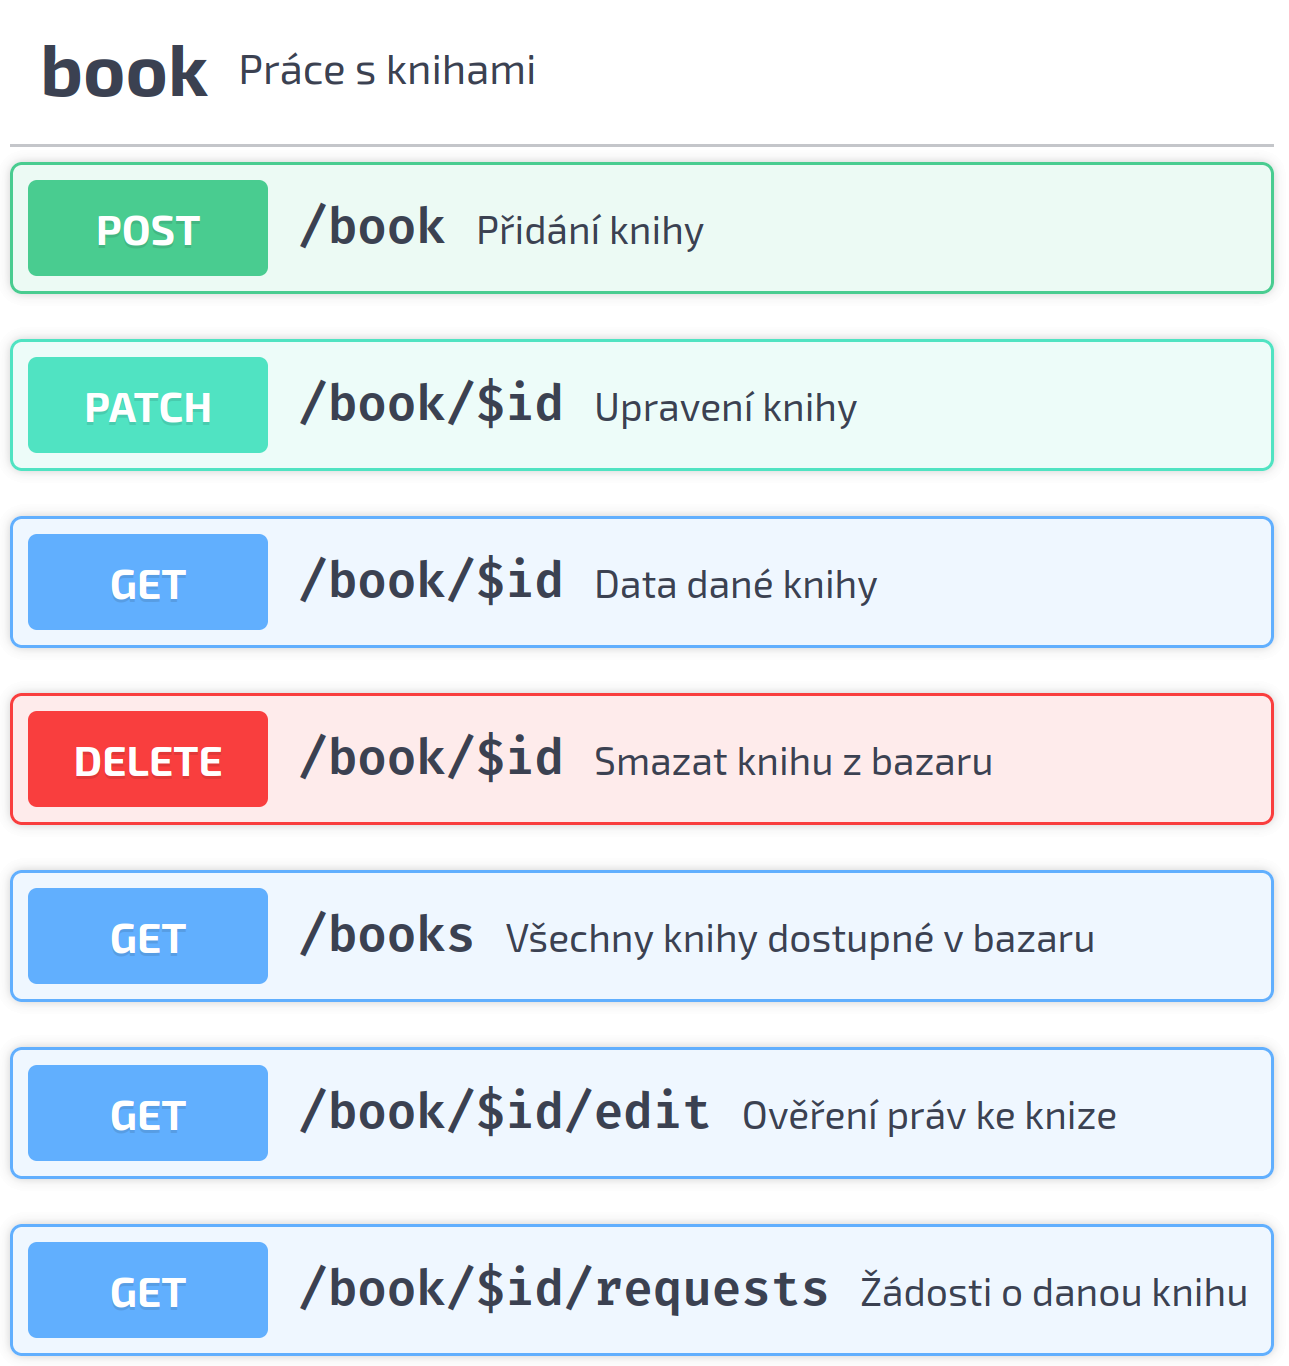
\includegraphics{../img/book.png}}
		\end{column}
		\begin{column}{.55\textwidth}
			\vspace{8.2mm}
			\scalebox{0.5}{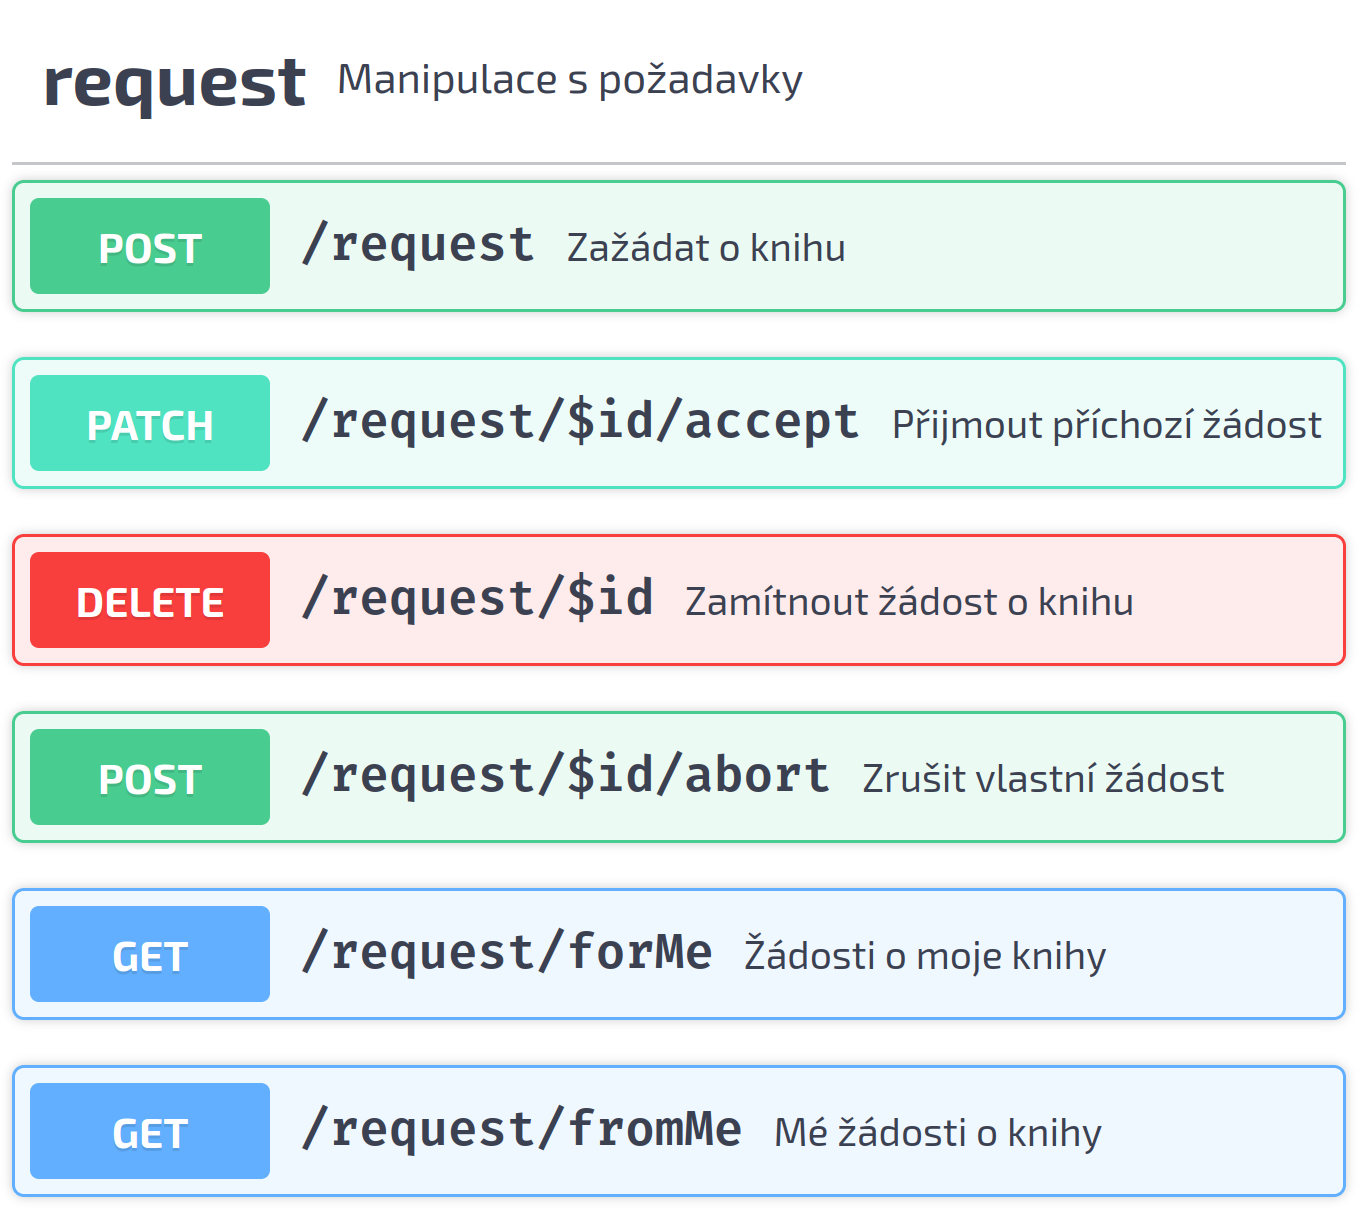
\includegraphics{../img/request.png}}
		\end{column}
	\end{columns}
}

\frame{
	\frametitle{Komunikace s databází}
	\begin{itemize}
		\item mariadb × mysql -- potíže s přihlášením
		\item přípojení přes \textit{factory} metodu
		\item \textit{wrapper}y na tabulky
	\end{itemize}
}

\frame{
	\frametitle{Emaily}
	\begin{columns}
		\begin{column}{.55\textwidth}
			\vspace{-1.6cm}
			\begin{itemize}
				\item jednotné zpracování
				\item modularitu
				\item uzpůsobeno běhu programu
				\item podle dat, která již víme
			\end{itemize}
		\end{column}
		\begin{column}{.35\textwidth}
			\vspace{-2mm}
			\scalebox{0.65}{
\includegraphics{../img/mail.png}}
		\end{column}
	\end{columns}
}

\section{Klient}
\frame{
	\frametitle{Struktura}
	\begin{itemize}
		\item záhlaví: logo, vyhledávací pole, účet \vbox{\hspace{1.305cm}
\includegraphics{../img/Header.png}\vspace{-2mm}}
		\item obsah stránky
			\begin{itemize}
				\item seznam inzerátů
				\item přidání inzerátu: formulář, náhled
				\item uživatel: I/O žádosti, seznam vlastnictví
			\end{itemize}
	\end{itemize}
}

\frame{
	\frametitle{Seznam knih}
	\begin{columns}
		\begin{column}{.535\textwidth}
			\vspace{-19.4mm}
			\begin{itemize}
				\item vyhledávání v záhlaví
				\item akce možné přihlášením
				\item zpětná reakce zabarvením
				\item majitel má jiné možnosti
			\end{itemize}
		\end{column}
		\begin{column}{.37\textwidth}
			\vspace{-3mm}
			\scalebox{0.55}{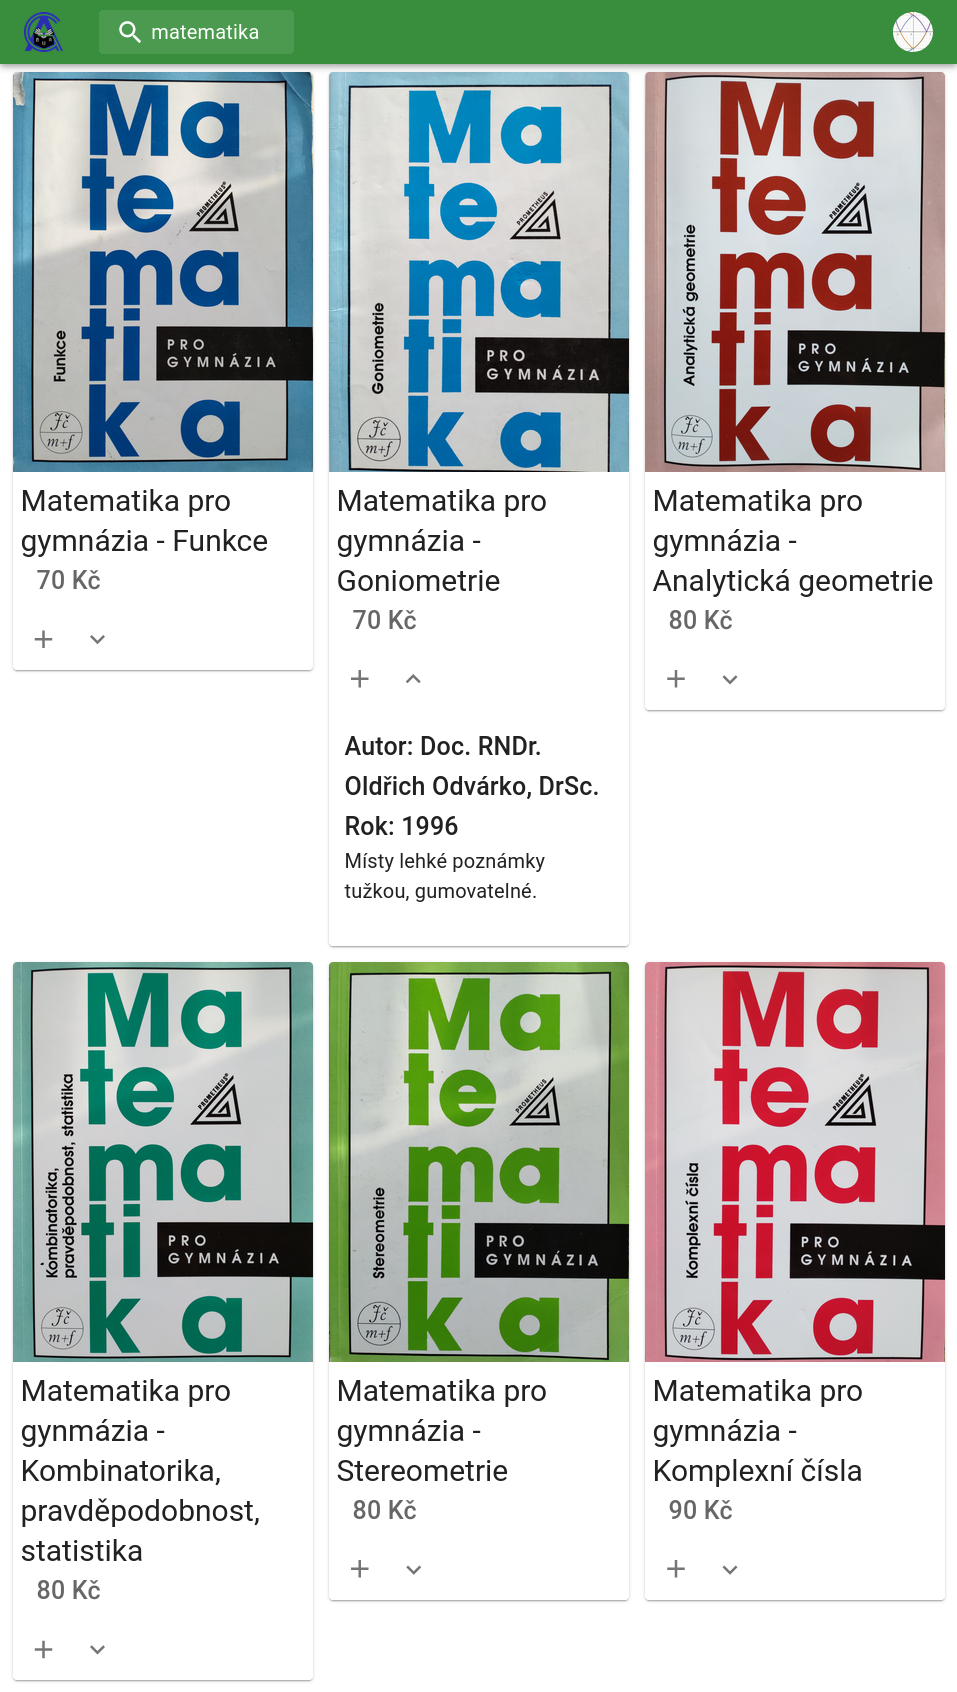
\includegraphics{../img/BookList.png}}
		\end{column}
	\end{columns}
}

\frame{
	\frametitle{Přidáni knihy}
	\begin{columns}
		\begin{column}{.525\textwidth}
			\vspace{-14.5mm}
			\begin{itemize}
				\item náhled výsledné podoby
				\item fotografie: \texttt{client-compress}
				\item server přes \texttt{multer}
				\item použito i na úpravy
			\end{itemize}
		\end{column}
		\begin{column}{.379\textwidth}
			\vspace{-8mm}
			\scalebox{0.8}{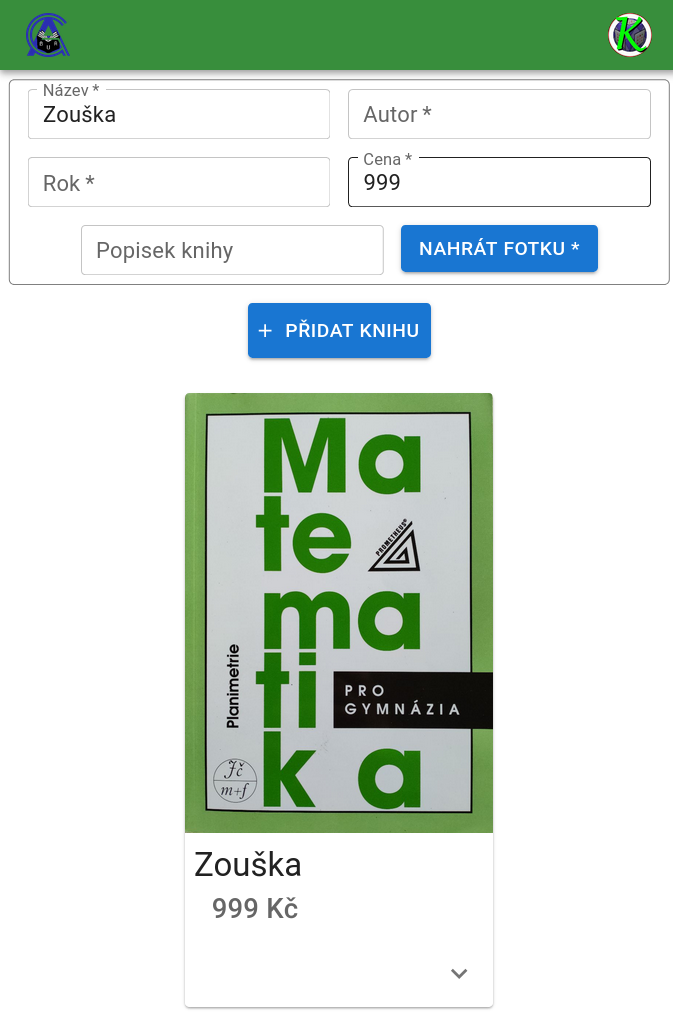
\includegraphics{../img/BookCommit.png}}
		\end{column}
	\end{columns}
}

\frame{
	\frametitle{Práce s žádostmi}
	\begin{columns}
		\begin{column}{.58\textwidth}
			\vspace{-16mm}
			\begin{itemize}
				\item řazení datem
				\item kontrola stavu
				\item zrušení možné obousměrně
				\item automatické skrytí ostatních
			\end{itemize}
		\end{column}
		\begin{column}{.325\textwidth}
			\vspace{-4.5mm}
			\scalebox{0.85}{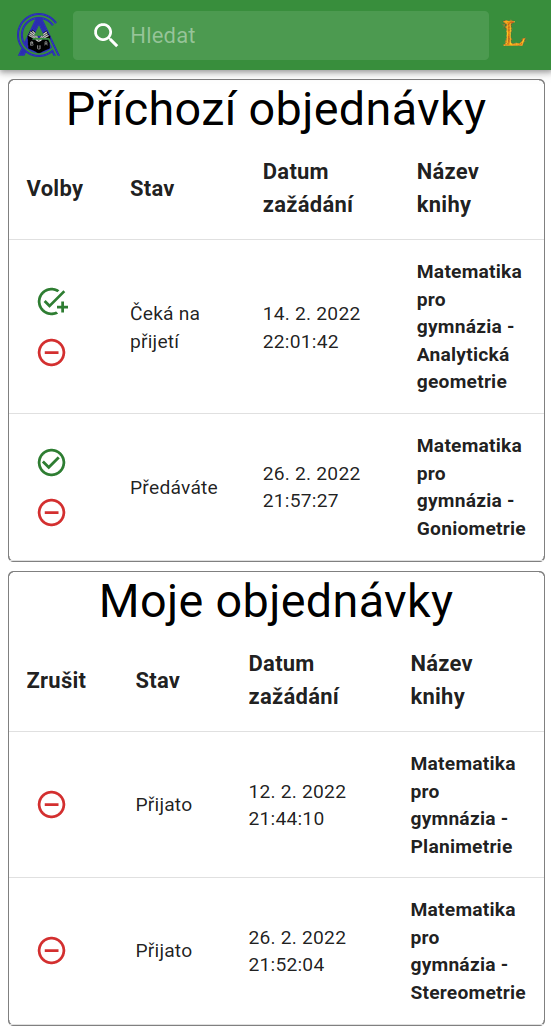
\includegraphics{../img/Requests.png}}
		\end{column}
	\end{columns}
}

\frame{
	\frametitle{Závěr}
	\section{Závěr}
	\begin{itemize}
		\item aplikace funguje
		\item \texttt{react} s globálním stavem
		\item bonusy byly uskutečnitelné
		\item malé vylepšováky na klienta
	\end{itemize}
}
\end{document}
